\documentclass{article}

\usepackage{amsmath}
\usepackage{graphicx}
\graphicspath{ {/home/vian/0_uam/1_TFG/latex/img} }

\title{Qiskit - Max Cut}
\date{}

\begin{document}
\maketitle{}

\begin{figure}[htbp]
  \centering
  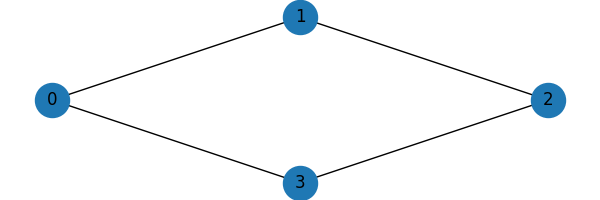
\includegraphics{qiskit_grafo/qiskit_grafo}
\end{figure}

\section{Problema de optimización Max Cut}

Dado un grafo, asignar a los nodos un valor 0 o 1 tal que se maximice el número de aristas del grafo entre nodos de distinto valor.

\section{Formulación del problema}

Sea G un grafo tal que: 
\begin{flalign*}
  &G = (V, E) \\
  &V = [0, 1, 2, 3] \\
  &E = [(0, 1), (1, 2), (2, 3), (0, 3)] \\
\end{flalign*}
Y sea \(x_i = 0, 1\) el valor asignado al nodo i.

\section{Formulación de \(H_p\)}
\begin{itemize}
\item Función de coste clásica:
  \begin{flalign*}
    C(x) = \sum_{(i, j) \in E} (x_i * (1 - x_j) + x_j * (1 - x_i))
  \end{flalign*}
  
\item Se realiza un cambio de variable tal que:
  \begin{flalign*}
    C(x) &\rightarrow g(z) \\
    x_i &\rightarrow \frac{1-z_i}{2} \\
    z_i &= \begin{cases}
             1  \text{ si } x_i = 0 \\
             -1 \text{ si } x_i = 1
           \end{cases} \\
  \end{flalign*}
  
  Entonces
  \begin{flalign*}
    g(z) &= \sum_{(i, j) \in E}[\frac{1 - z_i}{2} * (1 - \frac{1 - z_j}{2}) + \frac{1 - z_j}{2} * (1 - \frac{1 - z_i}{2})] =
           && \text{\footnotemark} \\
         &= \sum_{(i, j) \in E}\frac{1}{4}(2 - 2*z_i*z_j) = \sum_{(i, j) \in E}\frac{1 - z_i*z_j}{2}
  \end{flalign*}
  \footnotetext{Nota:
    \( \frac{1 - z_i}{2} * (1 - \frac{1 - z_j}{2}) =
    \frac{1 - z_i}{2} * \frac{1 - z_j}{2} =
    \frac{1}{4} * (1 - z_i + z_j - z_i*z_j) \)}

\item Problem hamiltonian: Sustituir variables en formato Ising (\(z_i = 1, -1\)) por puertas Pauli z en el qubit i (\(\sigma_{z}^{i}\)):
  \begin{flalign*}
    &H_p = \sum_{(i, j) \in E}\frac{1 - \sigma_{z}^{i} \otimes \sigma_{z}^{j}}{2} && \\
  \end{flalign*}

\item Operador unitario \(U(H_p, \gamma)\): \\
  Dada la definición de operador \(R_{zz_{i, j}}(\lambda) = exp(-i*\frac{\lambda}{2} * \sigma_{z}^{i} \otimes \sigma_{z}^{j} ) \)
  \begin{flalign*}
    U(H_p, \gamma) &= exp(-i * \gamma * H_p) = \prod_{(i, j) \in E}exp(-i * \gamma * \frac{1 - \sigma_{z}^{i} \otimes \sigma_{z}^{j}}{2}) = &&\\
              &= \prod_{(i, j) \in E} [exp(+i * \frac{\gamma}{2} *  \sigma_{z}^{i} \otimes \sigma_{z}^{j}) * exp(-i * \frac{\gamma}{2})] = && \text{\footnotemark} \\
              &= \prod_{(i, j) \in E} exp(-i * \frac{-\gamma}{2} *  \sigma_{z}^{i} \otimes \sigma_{z}^{j}) = \\
              &= \prod_{(i, j) \in E} R_{zz_{i, j}}(-\gamma)
  \end{flalign*}
  \footnotetext{La fase global es despreciable}

\item Operador unitario \(U(H_m, \gamma)\): \\
  El operador mixer hamiltonian (\(H_m\)) es el mismo para cualquier instancia de QAOA.
  \begin{flalign*}
    &R_{x_{i}}(\lambda) = exp(-i * \frac{\lambda}{2} * \sigma_x^i) &&\\
    &H_m = \sum_{i=0}^{|V|}\sigma_x^i \\
    &U(H_m, \beta) = exp(-i * \beta * H_m) = \prod_{i=0}^{|V|}exp(-i * \beta * \sigma_x^i) = \prod_{i=0}^{|V|}R_{x_{i}}(2* \beta) \\
  \end{flalign*}

\end{itemize}

\section{Resultados}

Dada la naturaleza del problema Max-Cut existen dos resultados óptimos: ``1010'' y ``0101'', que devuelven el máximo de la función de coste (\(C(x) = 4\)). Un valor ``abcd'' sería equivalente a dar un valor ``a'' al nodo 3, ``b'' al nodo 2 y así sucesivamente.

\begin{itemize}
\item Estadísticas
  % p = 1
  % MAX: ('0101': 0.51), ('1010': 0.49)
  % GLOBAL: ('1010', 0.260873046875) ('0101', 0.2605244140625) ('1001', 0.087294921875) ...
  % p = 2
  % MAX: ('1010': 0.507), ('0101': 0.493)
  % GLOBAL: ('1010', 0.49141796875) ('0101', 0.4902607421875) ('0011', 0.003029296875) ...
  % p = 3
  % MAX: ('0101': 0.47), ('1010': 0.53)
  % GLOBAL: ('0101', 0.481150390625) ('1010', 0.4798994140625) ('0110', 0.0069404296875) ...
  \begin{table}[htbp]
    \centering
    \begin{tabular}{|c|r|r|}
      \hline
      \textbf{nº Capas} & \textbf{Estadística máxima} & \textbf{Estadística global} \\ \hline
      p = 1 & 100\% & 52.14\% \\ \hline
      p = 2 & 100\% & 98.17\% \\ \hline
      p = 3 & 100\% & 96.10\% \\ \hline
      p = 4 & 100\% & 98.70\% \\ \hline
      p = 5 & 100\% & 98.90\% \\ \hline
    \end{tabular}
    \caption{Resultados de la ejecución del problema Max-Cut de Qiskit}
  \end{table}
  Según esta tabla, se encuentra el camino óptimo con cualquier número de capas el 100\% de las ejecuciones.

\item Funciones graficadas:
  \begin{figure}[htbp]
    \centering
    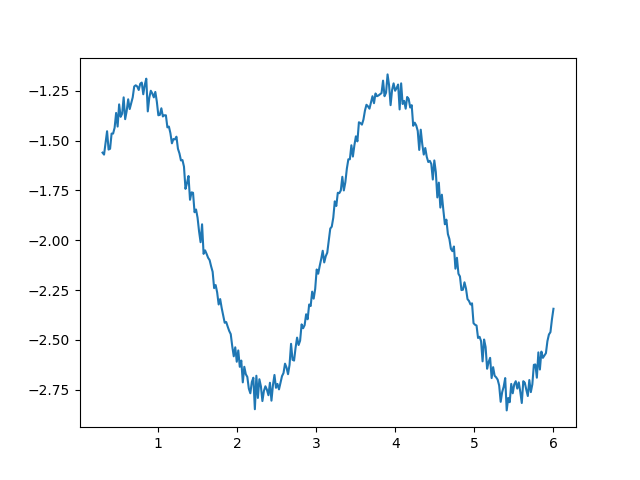
\includegraphics[scale=0.5]{qiskit_grafo/gamma_fun_2d}
    \caption{Función gamma con \(\beta = 1.0\) y variando \(\gamma\)}
  \end{figure}
  \begin{figure}[htbp]
    \centering
    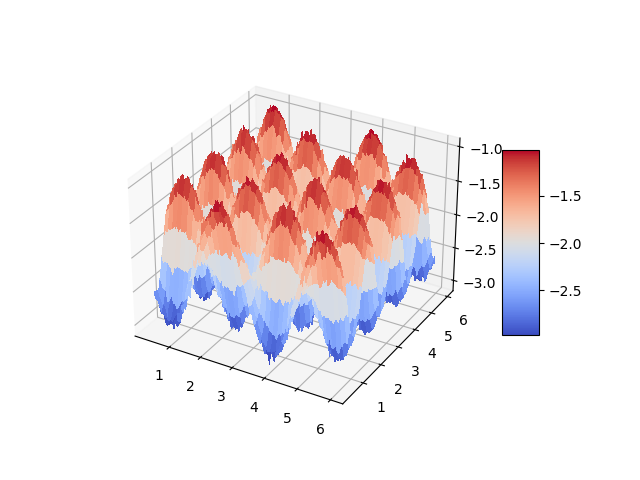
\includegraphics[scale=0.5]{qiskit_grafo/gamma_fun_3d}
    \caption{Función variando \(\beta, \gamma\)}
  \end{figure}
\end{itemize}

\end{document}

%%% Local Variables:
%%% mode: latex
%%% TeX-master: t
%%% End:
